This work brings together Bayesian practice and functional programming theory, and bridges them using measure-theoretic probability.

In this chapter, we attempt to give enough background to motivate and explain Bayesian practice and functional programming theory.
We only \emph{motivate} measure-theoretic probability here.
Further on, we introduce, explain and use parts as we need them.

It is difficult to find two areas in computer science as different as Bayesian practice and functional programming theory.
In Bayesian practice, we find deeply held belief that unknowns can and should be \emph{quantified} (by probabilities), reasoning by probabilistic inference, willingness to accept many kinds of approximations, and common notation that is---to put it kindly---flexible.
In functional programming theory, we find deeply held belief that unknowns should be \emph{qualified} (usually universally), reasoning by logical inference, little tolerance for unsound approximations even if they converge, and common notation that is---to put it kindly---almost precise enough to feed to a compiler.

There is one common trait that makes bridging both areas even conceivable.
While Bayesians model processes and functional programming researchers model languages, both approach their tasks methodically, and both create theories in which every entity they want to reason about is represented explicitly.
If something important is going on behind the scenes---whether a hidden Markov process or mutating the program's store---it is brought to the fore and fully characterized.
In both areas, the extra time and cognitive burden are considered worthwhile payment for reliable artifacts and repeatable results.

It is this trait---explicit representation---that makes it possible to automate Bayesian inference, and again this trait that makes it possible to prove the automation correct.


\section{Bayesian Practice}

From Bayesian practice, the requisite background knowledge includes probability mass functions, probability densities, queries and manipulation rules, Bayesian modeling, and Bayesian inference.
We assume readers know arithmetic, some set theory, functions, and the basic ideas behind integration.

\subsection{Discrete Probability and Joint Distribution Models}

In a probabilistic model of a real-world process, there are distinguished identifiers that denote random values, called \keyword{random variables}.
These are regarded as free variables, but with additional information that quantifies the likelihoods of the values they may take on.
The additional information is completely characterized by a function called a \keyword{joint distribution}.

For example, suppose $X,Y \in \set{h,t}$ are random variables that represent the \emph{observable} outcomes of coin tosses.
Further, let the joint distribution $p_{X,Y} : \set{h,t} \times \set{h,t} \to [0,1]$ quantify the likelihood of every possible combination of observable outcomes by defining
\begin{equation}
	p_{X,Y}\ =\ \left[(h,h) \mapsto \frac{1}{4},
		(h,t) \mapsto \frac{1}{4},
		(t,h) \mapsto \frac{1}{6},
		(t,t) \mapsto \frac{1}{3}\right]
\end{equation}
(The subscript ``$X,Y$'' is just part of the function name, and has no special meaning.)
This is a \keyword{probability mass function}: its outputs sum to $1$.

The probability that $X = t$ and $Y = h$ is $p_{X,Y}(t,h) = \frac{1}{6}$.
Another way to write ``the probability that $X = t$ and $Y = h$'' is with a \keyword{probability query}:
\begin{equation}
	\Pspec{X = t \band Y = h}\ =\ p_{X,Y}(t,h)
\end{equation}
A probability query always implicitly refers to some ambient joint distribution.
In general, the result of a probability query $\Pspec{e}$ is the sum of probabilities of observable outcomes for which $e$ is true.
Conjunctions are often separated by a comma; e.g. $\Pspec{X = x, Y = y} = \Pspec{X = x \band Y = y}$.

Probability queries have manipulation rules.
One is that random variables may be ``summed out'' to consider the probabilities of the values of others independently.
For example, to consider just the probabilities of values of $X$, we may sum out $Y$:
\begin{equation}
	\Pspec{X = x}\ =\ \sum_{y \in \set{h,t}} \Pspec{X = x, Y = y}
\end{equation}
According to this rule, $X$ represents the outcome of a fair coin toss (independent of $Y$):
\begin{equation}
\begin{aligned}
	\Pspec{X = h}&\ =\ \Pspec{X = h, Y = h} + \Pspec{X = h, Y = t}\ =\ \frac{1}{4} + \frac{1}{4}&=\ \frac{1}{2}
\\
	\Pspec{X = t}&\ =\ \Pspec{X = t, Y = h} + \Pspec{X = t, Y = t}\ =\ \frac{1}{6} + \frac{1}{3}&=\ \frac{1}{2}
\end{aligned}
\end{equation}

Another manipulation rule allows fixing the value of one random variable to consider the probabilites of the values of others \emph{dependently}.
For example, if $x$ is fixed and $\Pspec{X = x} > 0$, then the probability that $Y = y$ is
\begin{equation}
	\Pspec{Y = y \given X = x}\ =\ \frac{\Pspec{X = x,Y = y}}{\Pspec{X = x}}
\end{equation}
This \keyword{conditional probability} query is read ``the probability that $Y = y$ \emph{given} $X = x$.''
Using this rule, we can determine that, if $X$ is known to be $t$, then $Y$ represents a coin toss that is not fair:
\begin{equation}
\begin{aligned}
	\Pspec{Y = h \given X = t}&\ =\ \frac{\Pspec{X = t,Y = h}}{\Pspec{X = t}}\ =\ \frac{\frac{1}{6}}{\frac{1}{2}}&=\ \frac{1}{3}
\\
	\Pspec{Y = t \given X = t}&\ =\ \frac{\Pspec{X = t,Y = t}}{\Pspec{X = t}}\ =\ \frac{\frac{1}{3}}{\frac{1}{2}}&=\ \frac{2}{3}
\end{aligned}
\end{equation}
We could similarly show $\Pspec{Y = h \given X = h} = \frac{1}{2}$ and $\Pspec{Y = t \given X = h} = \frac{1}{2}$, so when $X$ is known to be $h$, $Y$ represents a fair coin toss.

To avoid the condition $\Pspec{X = x} > 0$, the preceeding rule is often written
\begin{equation}
\begin{aligned}
	\Pspec{X = x, Y = y}&\ =\ \Pspec{X = x} \cdot \Pspec{Y = y \given X = x} \\
	&\ =\ \Pspec{Y = y} \cdot \Pspec{X = x \given Y = y}
\end{aligned}
\end{equation}
In this form, it is called the \keyword{chain rule}.

As a function of $x$, $\Pspec{X = x}$ is a probability mass function, but over just $X$ instead of $X$ and $Y$ together.
With any fixed $x$, as a function of $y$, $\Pspec{Y = y \given X = x}$ is also a probability mass function.
Most Bayesian models are constructed by reifying these queries as functions called (respectively) \keyword{distributions} and \keyword{conditional distributions}, and using the chain rule to build a joint distribution.
For the present example,
\begin{equation}
\begin{aligned}
	p_X&\ =\ \left[h \mapsto \frac{1}{2}, t \mapsto \frac{1}{2}\right]
\\
	p_{Y|X}(y \given x)&\ =\
	\begin{cases}
		x = h & \left[h \mapsto \frac{1}{2}, t \mapsto \frac{1}{2}\right](y) \\
		x = t & \left[h \mapsto \frac{1}{3}, t \mapsto \frac{2}{3}\right](y)
	\end{cases}
\\
	p_{X,Y}(x,y)&\ =\ p_X(x) \cdot p_{Y|X}(y \given x)
\end{aligned}
\end{equation}
In the conditional distribution $p_{Y|X}$, the ``$Y|X$'' subscript is simply part of the function name, and in applying it, $(y \given x)$ is just another way to write the arguments $(y,x)$.\footnote{It is common to leave off subscripts such as $Y|X$ and use the form of application to distinguish the different $p$s; e.g. $p(x)$ means $p_X(x)$ and $p(y \given x)$ means $p_{Y|X}(y \given x)$. Doing so is helpful when there are many random variables, and it is usually unambiguous, but the practice often confuses and frustrates newcomers.}
The syntax simply connotes that we expect $\Pspec{Y = y \given X = x}\ =\ p_{Y|X}(y \given x)$.

This model can be more compactly specified by a constructive theory about $X$ and $Y$, which states only the properties that a joint distribution model must satisfy:
\begin{equation}
\begin{aligned}
	X&\ \sim\ \left[h \mapsto \frac{1}{2}, t \mapsto \frac{1}{2}\right]
\\
	Y&\ \sim\ 
	\begin{cases}
		X = h & \left[h \mapsto \frac{1}{2}, t \mapsto \frac{1}{2}\right] \\
		X = t & \left[h \mapsto \frac{1}{3}, t \mapsto \frac{2}{3}\right]
	\end{cases}
\end{aligned}
\end{equation}
Here, $X \sim e$ is read ``$X$ is distributed $e$.''
In this leaner form, it is perhaps easier to understand the process being modeled, which is
\begin{enumerate}
	\item Toss a coin and call its outcome $X$.
	\item If $X = h$, toss a fair coin and call its outcome $Y$.
	\item If $X = t$, toss a biased coin with heads probability $\frac{1}{3}$ and call its outcome $Y$.
\end{enumerate}
It is usually easy to manually translate constructive theories into programs that sample random variable values.

By combining a conditional probability query and the chain rule (or using the chain rule twice), we get \keyword{Bayes' law}: if $\Pspec{Y = y} > 0$, then
\begin{equation}
	\Pspec{X = x \given Y = y}\ =\ \frac{\Pspec{X = x} \cdot \Pspec{Y = y \given X = x}}{\Pspec{Y = y}}
\end{equation}
This is different than $\Pspec{Y = y \given X = x}$.
This time, we are interested in the conditional probability that $X = x$ given we know $Y = y$ for some fixed $y$.

For example, suppose we did not observe $X$, but were allowed to observe $Y = t$.
Given that we know the second coin toss is tails, the probability that $X = t$ is
\begin{equation}
\begin{aligned}
	\Pspec{X = t \given Y = t}&\ =\ \frac{\Pspec{X = t} \cdot \Pspec{Y = t \given X = t}}{\Pspec{Y = t}}
\\
	&\ =\ \frac{\frac{1}{2} \cdot \frac{2}{3}}{\sum_{x \in \set{h,t}} \Pspec{X = x, Y = t}}
\\
	&\ =\ \frac{\frac{1}{2} \cdot \frac{2}{3}}{\frac{1}{4} + \frac{1}{3}}
	\ =\ \frac{\frac{1}{3}}{\frac{7}{12}}
	\ =\ \frac{4}{7}
\end{aligned}
\end{equation}
which is greater than $\Pspec{X = t} = \frac{1}{2}$.
Similarly, $\Pspec{X = h \given Y = t} = \frac{3}{7}$, which is less than $\Pspec{X = h} = \frac{1}{2}$.
Observing the effects of the first coin toss---even random effects---allows us to draw stronger conclusions about the first coin toss.
In this case, we know it is more likely to be tails.

Using Bayes' law to draw probabilistic conclusions about probabilistic processes given observed probabilistic effects is called \keyword{Bayesian inference}.

It is easy for probability newcomers with logical background to think of conditional queries as a fuzzy kind of logical implication.
A short example demonstrates that doing so leads to faulty intuition.
To compute the probability that $Y = t \implies X = t$, we apply logical rules to the query until it is a disjunction of distinct observable outcomes, and add their probabilities:
\begin{equation}
\begin{aligned}
	\Pspec{Y = t \implies X = t}
	&\ =\ \Pspec{\neg (Y = t) \bor X = t}
\\
	&\ =\ \Pspec{Y = h \bor X = t}
\\
	&\ =\ \Pspec{(Y = h \band X = t) \bor (Y = h \band X = h) \bor (Y = t \band X = t)}
\\
	&\ =\ \Pspec{Y = h \band X = t} + \Pspec{Y = h \band X = h} + \Pspec{Y = t \band X = t}
\\
	&\ =\ \frac{1}{6} + \frac{1}{4} + \frac{1}{3} \ =\ \frac{3}{4}
\end{aligned}
\end{equation}
This is clearly not $\Pspec{X = t \given Y = t} = \frac{4}{7}$.
In a similar fashion, $\Pspec{Y = t \implies X = h} = \frac{2}{3}$, which is not $\Pspec{X = h \given Y = t} = \frac{3}{7}$.

In conditioning on $Y = t$, we did not consider any outcomes in which $Y \neq t$: we restricted the possible outcomes to those for which $Y = t$ and renormalized the probabilities of $X = h$ and $X = t$.
On the other hand, in computing the probability that $Y = t \implies X = t$, we had to consider \emph{all} of the outcomes in which $Y \neq t$, and only \emph{one} outcome in which $Y = t$.


\subsection{Probability Densities and Density Models}

Probability mass functions cannot quantify the likelihoods of uncountably many observable outcomes, such as when $X \in \Re$.
In these cases, the distributions, conditional distributions, and joint distributions are specified using \keyword{probability density functions}: functions over outcomes that \emph{integrate} to $1$ instead of sum to $1$.\footnote{For readers familiar with measure theory: we use the word \emph{density} for densities with respect to Lebesgue measure, and \emph{mass} for densities with respect to counting measure. We call all other densities \emph{derivatives}.}

\begin{figure*}[tb]\centering
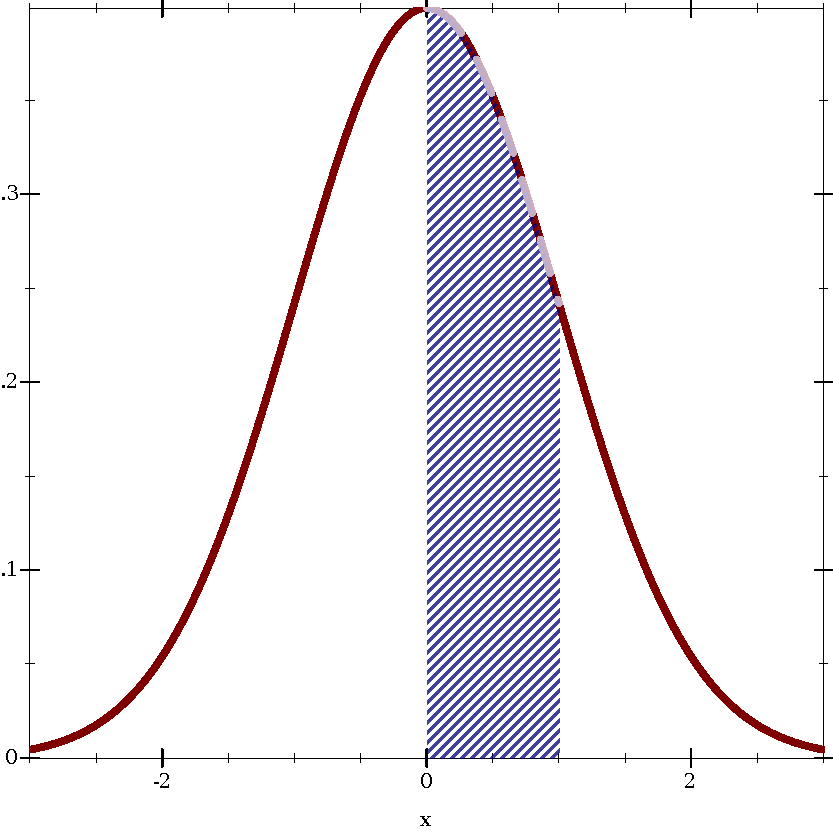
\includegraphics[width=4in]{density-integrate}
\caption[Computing probabilities using the standard normal density function]{Integrating under the standard normal density to compute $\Pspec{X \in (0,1)} \approx 0.34$.}
\label{fig:density-integrate}
\end{figure*}

For example, this probability density function defines the \keyword{standard normal distribution}, or bell curve:
\begin{equation}
	f_N(x)\ =\ \frac{1}{\sqrt{2\pi}} \exp\left(-\frac{x^2}{2}\right)
\end{equation}
If $X$ has a standard normal distribution, then the probability that $X \in (0,1)$ is
\begin{equation}
	\Pspec{X \in (0,1)}\ =\ \int_0^1 f_N(x)\,dx\ \approx\ 0.3413447460685
\end{equation}
Figure~\ref{fig:density-integrate} plots this density and illustrates integrating under it to compute $\Pspec{X \in (0,1)}$.

When probabilities are computed by integrating density functions, sets of outcomes may have positive probability, but every \emph{single} outcome has zero probability.
For any random variable $X \in \Re$, outcome $x \in \Re$, and density function $f_X : \Re \to [0,+\infty)$,
\begin{equation}
	\Pspec{X = x}\ =\ \int_x^x f_X(x)\, dx\ =\ (f_X(x) - 0) \cdot (x - x)\ =\ f_X(x) \cdot 0\ =\ 0
\end{equation}
As a consequence, interval endpoints do not matter; i.e. $\Pspec{X \in [a,b]}\ =\ \Pspec{X \in (a,b)}$.
We discuss other, more difficult consequences further on.

The normal distribution can be extended to a \keyword{distribution family} by parameterizing it on a \emph{location} $\mu$ and a \emph{scale} $\sigma$:
\begin{equation}
	f_N(x \given \mu,\sigma)\ =\ \frac{1}{\sigma\sqrt{2\pi}} \exp\left(-\frac{(x-\mu)^2}{2\sigma^2}\right)
\end{equation}
A normal distribution's location $\mu$ and scale $\sigma$ are also known as its \emph{mean} and \emph{standard deviation}, respectively.

\begin{figure*}[tb]\centering
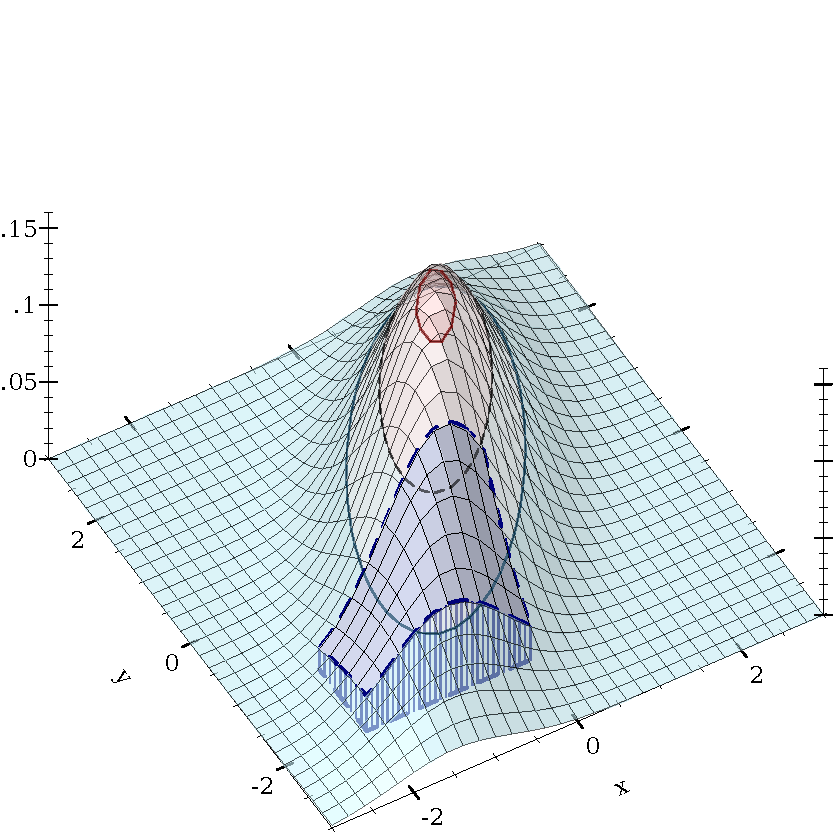
\includegraphics[width=4in]{2d-density-integrate}
\caption[Joint density model plot]{The joint density model $f_{X,Y}$ constructed from the density $f_X$ and the conditional density $f_{Y|X}$. Integrating under $f_{X,Y}$ on the set $(-2,0) \times (-2,-1)$ computes $\Pspec{X \in (-2,0), Y \in (-2,-1)}$.}
\label{fig:joint-density-model}
\end{figure*}

Using parameterized distributions, we can define a \keyword{joint density model} of a probabilistic process involving two random variables $X,Y \in \Re$:
\begin{equation}
\begin{aligned}
	f_X(x)&\ =\ f_N(x \given 0,1) \\
	f_{Y|X}(y \given x)&\ =\ f_N(y \given x,1) \\
	f_{X,Y}(x,y)&\ =\ f_X(x) \cdot f_{Y|X}(y \given x)
\end{aligned}
\end{equation}
Integrating under $f_{X,Y}$ computes probability queries:
\begin{equation}
	\Pspec{X \in (a,b), Y \in (c,d)}\ =\ \int_a^b \int_c^d f_{X,Y}(x,y)\,dy\,dx
\end{equation}
Figure~\ref{fig:joint-density-model} illustrates the joint density model $f_{X,Y}$ and computing a probability query.

As with discrete models, density models can be specified by constructive theories:
\begin{equation}
\begin{aligned}
	X&\ \sim\ \mathrm{Normal}(0,1) \\
	Y&\ \sim\ \mathrm{Normal}(X,1)
\end{aligned}
\end{equation}
The probabilistic process being modeled is
\begin{enumerate}
	\item Choose $X$ according to the standard normal distribution.
	\item Choose $Y$ according to the normal distribution with mean $X$, standard deviation $1$.
\end{enumerate}
Again, it is usually easy to manually translate such theories into programs that sample random variable values.

When all single outcomes have zero probability, interpreting theories in terms of expected conditional probability queries is difficult.
(In fact, doing so requires measure theory.)
Fortunately, densities have rules analogous to rules for manipulating probability queries, which allow practitioners to derive joint density models from theories and compute a restricted class of conditional queries.
Instances of the two most important rules are
\begin{equation}
\begin{aligned}
	f_{X}(x)&\ =\ \int_{-\infty}^{+\infty} f_{X,Y}(x,y)\,dy
\\
	f_{X,Y}(x,y)&\ =\ f_{X}(x) \cdot f_{Y|X}(y \given x)\ =\ f_{Y}(y) \cdot f_{X|Y}(x \given y)
\end{aligned}
\end{equation}
The second rule is the \keyword{chain rule for densities}, and it justifies constructing the joint density $f_{X,Y}$ from the density $f_X$ and the conditional density $f_{Y|X}$.

The rules for densities can be used to derive \keyword{Bayes' law for densities}: if $f_Y(y) > 0$, then, starting from the right-hand side of the chain rule,
\begin{equation}
\begin{aligned}
	f_{Y}(y) \cdot f_{X|Y}(x \given y)&\ =\ f_{X}(x) \cdot f_{Y|X}(y \given x)
\\
	f_{X|Y}(x \given y)&\ =\ \frac{f_{X}(x) \cdot f_{Y|X}(y \given x)}{f_{Y}(y)}
\\
	&\ =\ \frac{f_{X}(x) \cdot f_{Y|X}(y \given x)}{\displaystyle\int_{-\infty}^{+\infty} f_{X,Y}(x,y)\,dx}
\\
	&\ =\ \frac{f_{X}(x) \cdot f_{Y|X}(y \given x)}{\displaystyle\int_{-\infty}^{+\infty} f_{X}(x) \cdot f_{Y|X}(y \given x)\,dx}
\end{aligned}
\end{equation}
The last form is conveniently in terms of $f_{X}$ and $f_{Y|X}$, which we have on-hand.

Using Bayes' law for densities, we can draw conclusions about $X$ given knowledge about $Y$.
For example, suppose we want to know the distribution of $X$ given $Y = 2$, as a density.
A quite lengthy derivation finally results in
\begin{equation}
\begin{aligned}
	f_{X|Y}(x \given 2)&\ =\ \frac{f_{X}(x) \cdot f_{Y|X}(2 \given x)}{\displaystyle\int_{-\infty}^{+\infty} f_{X}(x) \cdot f_{Y|X}(2 \given x)\,dx}
\\
	&\ =\ \frac{f_N(x \given 0,1) \cdot f_N(2 \given x,1)}{\displaystyle\int_{-\infty}^{+\infty}
	f_N(x \given 0,1) \cdot f_N(2 \given x,1)\,dx}
\\
	&\,\,\cdots\ 
\\
	&\ =\ f_N(x \given 1, \sqrt{\tfrac{1}{2}})
\end{aligned}
\end{equation}
We can answer conditional probability queries by integrating $f_{X|Y}(x \given 2)\ =\ f_N(x \given 1, \sqrt{\tfrac{1}{2}})$:
\begin{equation}
	\Pspec{X \in (a,b) \given Y = 2}\ =\ \int_a^b f_N(x \given 1, \sqrt{\tfrac{1}{2}})\,dx
\end{equation}

\begin{figure*}[tbp]\centering
\subfloat[The original joint density model.]{
\label{fig:bayes-densities:1}
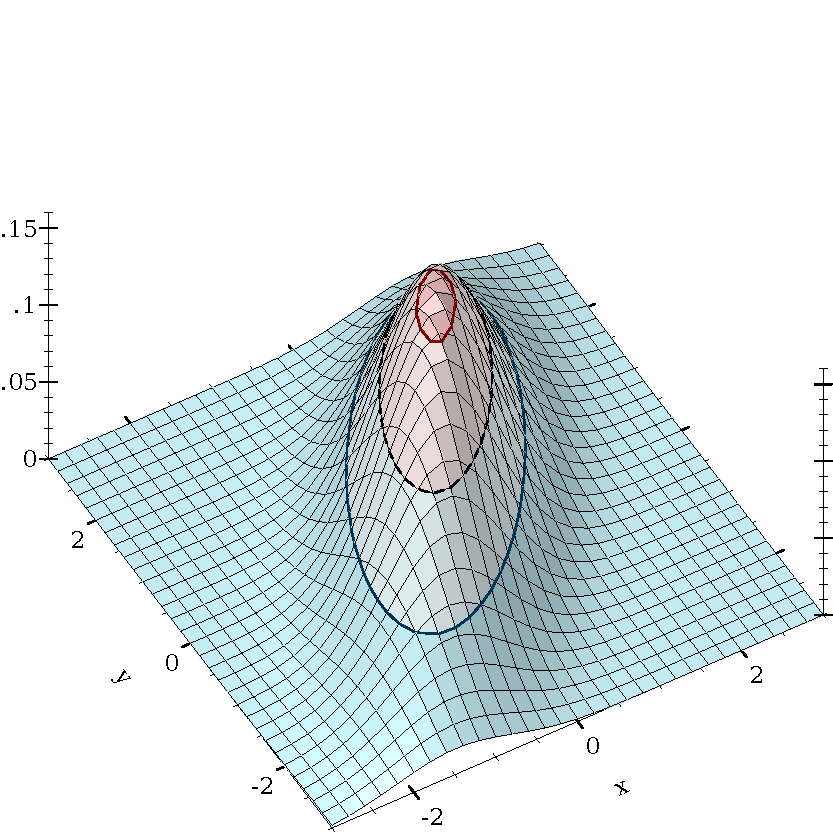
\includegraphics[width=3in]{bayes-densities-1}
}
\tab
\subfloat[Restricting the model to the subset of its domain where $y = 2$. The probability of the subset is zero.]{
\label{fig:bayes-densities:2}
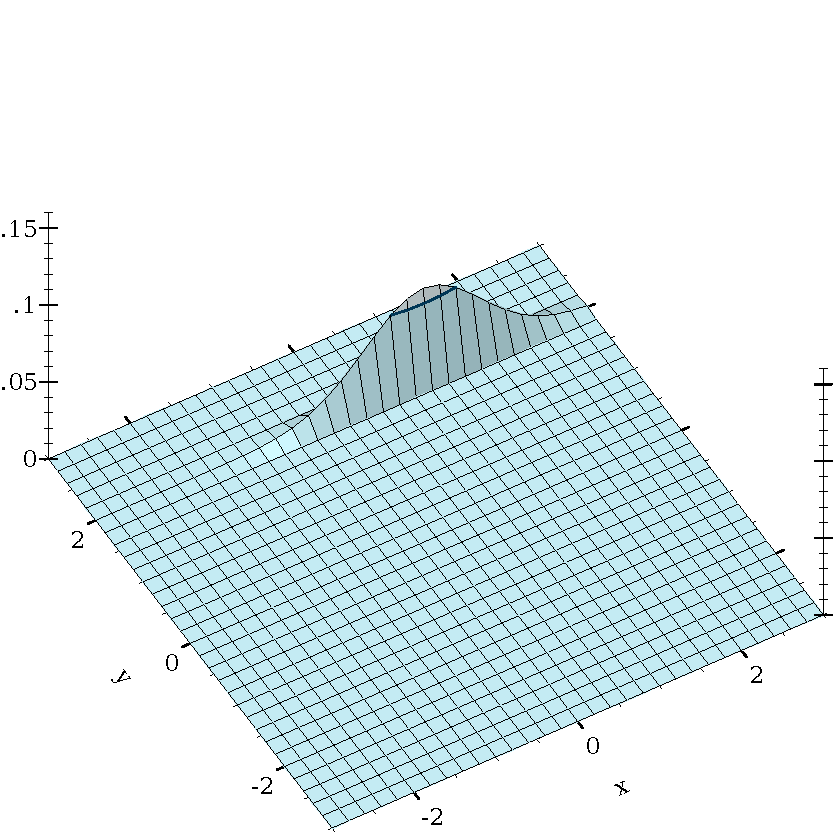
\includegraphics[width=3in]{bayes-densities-2}
}
\vspace{\baselineskip}

\subfloat[Projecting the restricted model onto the $x$ axis results in a density that integrates to a nonzero constant that is less than $1$.]{
\label{fig:bayes-densities:3}
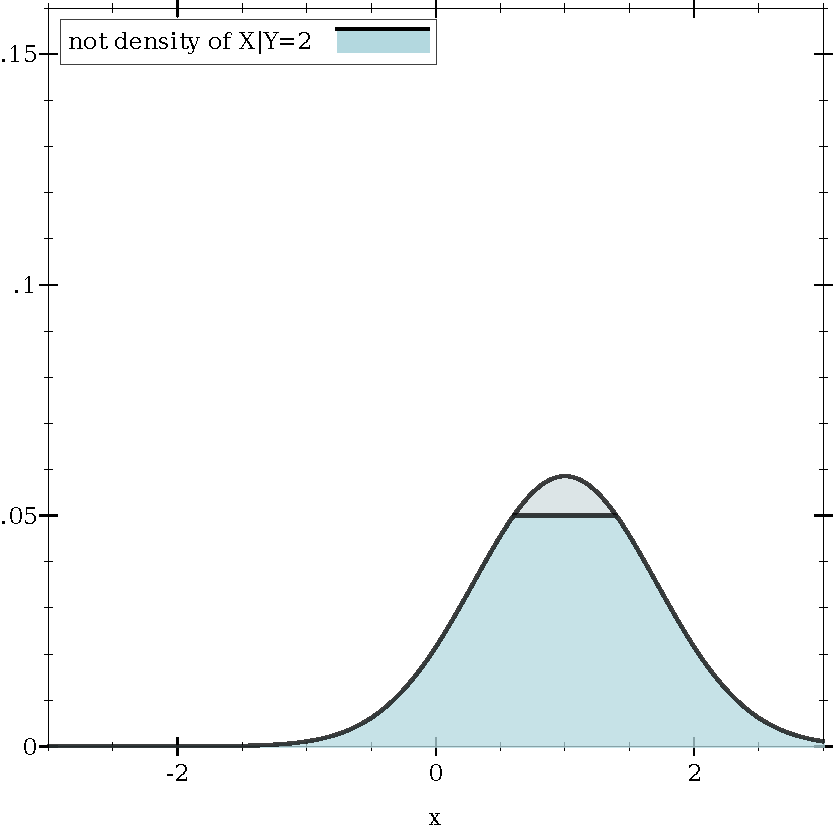
\includegraphics[width=3in]{bayes-densities-3}
}
\tab
\subfloat[Normalizing the restricted, projected model results in a probability density that characterizes the distribution of $X$ given $Y = 2$.]{
\label{fig:bayes-densities:4}
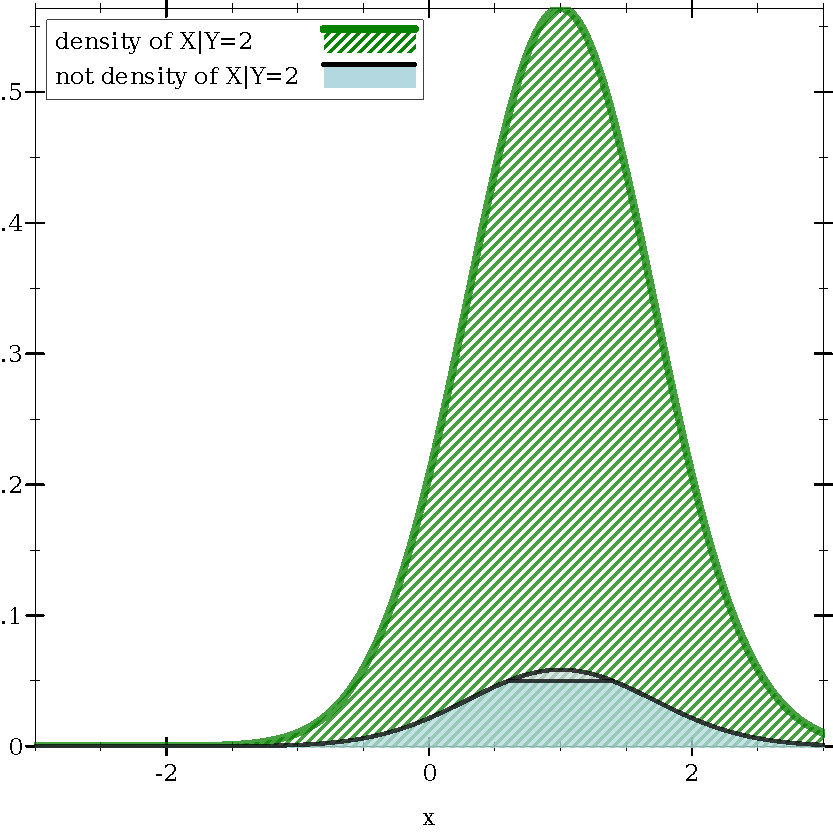
\includegraphics[width=3in]{bayes-densities-4}
}
\caption[Bayes' law for densities, in pictures]{Bayes' law for densities, in pictures.}
\label{fig:bayes-densities}
\end{figure*}

While using Bayes' law for densities is difficult, it is easy to visualize, at least in two dimensions.
We may think of its application as happening in three steps: restrict, project, then renormalize.
\figref{fig:bayes-densities} illustrates them.
First, we restrict the joint density model (\figref{fig:bayes-densities:1}) to the subset of $\Re \times \Re$ where $y = 2$ (\figref{fig:bayes-densities:2}).
Second, because the resulting model integrates to zero and therefore all answers to probability queries using it would be zero, we project it onto the $x$ axis (\figref{fig:bayes-densities:3}), on which it integrates to a positive value.
Third, because the total probability is now less than $1$, we renormalize the restricted, projected model by dividing its output by its area, and obtain a probability density (\figref{fig:bayes-densities:4}).

Using Bayes' law for densities is not only often technically challenging, but in general there are no closed-form solutions.
In such cases, practitioners turn to Monte Carlo integration, or sampling, to answer conditional probability queries.


\subsection{Motivating Measure-Theoretic Models}

It is easy to define a random variable whose distribution cannot be characterized by a density.
Suppose we have a thermometer whose output is not quite correct, but is usually within $1$ degree.
We could model the error with a normal distribution with standard deviation $1$.
If the thermometer cannot show a number greater than $100$ and we want to model that fact, assuming the correct temperature is $99$, we could write a theory about it like this:
\begin{equation}
\begin{aligned}
	T'&\ \sim\ \mathrm{Normal}(99,1) \\
	T&\ =\ \min(T',100)
\end{aligned}
\end{equation}
$T' \ge 100$ if and only if $T = 100$.
Therefore, $\Pspec{T' \ge 100} = \Pspec{T = 100} > 0$.
But we know that if $T$ has a density, $\Pspec{T = 100} = 0$.

Even though $T$ has no density, it must have a distribution, because $T \in (a,b)$ for any interval $(a,b)$ has a sensible probability, which we can compute by integrating the density of $T'$ up to $100$ and adding $\Pspec{T' \ge 100}$ if the interval happens to contain $100$:
\begin{equation}
	\Pspec{T \in (a,b)}\ =\ \int_{\min(a,100)}^{\min(b,100)} f_N(x \given 99,1)\,dx +
	\begin{cases}
		100 \in (a,b) & \Pspec{T' \ge 100} \\
		100 \notin (a,b) & 0
	\end{cases}
\end{equation}
Further, it is easy to write a program that samples $T$ values, and we expect the outputs of such programs to have well-defined probability distributions.

Another way to define a distribution that cannot be characterized by a density is to restrict a joint density model with a non-axial condition.
For example, with the present theory and model for $X,Y \in \Re$, suppose we want to answer questions like
\begin{equation}
	\Pspec{X \in (a,b),Y \in (c,d) \given \sqrt{X^2 + Y^2} = 1}
\end{equation}
which restricts the model to a unit circle.
To do so with a density, we need $f_{X,Y|\sqrt{X^2+Y^2}}(x,y \given z)$.
But for any $z$, a joint density for $X,Y$ restricted to $\sqrt{X^2+Y^2} = z$ cannot exist because the area of that circular set is zero.

In the preceeding examples, on a part of the distribution's domain that has length or area $0$ (i.e. the single outcome $100$ or the set $\setb{x \in \Re, y \in \Re}{\sqrt{x^2+x^2} = z}$), the probability of that set is nonzero.
Integrating on such a set can yield only $0$, so the distributions cannot be defined by densities.

There are many more sensible distributions that cannot be defined by densities, such as the distribution of a random variable $X \in \Re \u \Re^2$ or $X \in \Re^\Nat$.
Not only do sets of outcomes have sensible probabilities, but as in the thermometer example, \emph{it is easy to define random variables with these distributions}.

Measure theory's answer to this shocking lack of densities is to define probability distributions using \keyword{probability measures}, which map \emph{sets to probabilities} instead of \emph{values to instantaneous changes} in probability.
The measure defining $T$'s distribution directly answers queries such as $\Pspec{T \in (a,b)}$.
There is also a measure defined on sets of $\Re \times \Re$ that directly answers queries such as $\Pspec{X \in (a,b),Y \in (c,d) \given \sqrt{X^2 + Y^2} = 1}$.
Probability measures exist on spaces with varying and infinite dimension.

Chapter~\ref{ch:countable-models} introduces measure theory by using it to interpret discrete Bayesian theories mechanically.
Chapter~\ref{ch:preimage1} gives a measure-theoretic interpretation of probabilistic programs, which can encode Bayesian theories that do not have density models.


\begin{comment}
The greatest commonality in the two sides is the attitude with which they approach modeling.
While Bayesian practitioners model processes and functional programming researchers model languages, both approach their tasks methodically, and both create models in which every entity they want to reason about is represented explicitly---sometimes painfully so.
Both sides trust their explicit models to lead to more reliable artifacts and repeatable results than models created by other means.

Therefore, for us, choosing a side to target for publication comes down to determining which side's venues will tolerate the precision necessary to explicitly define our models.
At this stage, in which we almost exclusively model languages, it is clear that we must choose functional programming.
Thus, most of this dissertation assumes readers are functional programming researchers, and tutors them in the necessary Bayesian background.

For readers who are not functional programming researchers, we present this overview of the relevant functional programming theory, and beg their indulgence as we use it to model languages with enough precision to make our artifacts reliable and our results repeatable.

We assume readers know basic computer science theory, including propositional logic, relations, functions, proof by induction, context-free grammars, and nondeterminism.

\end{comment}

\section{Functional Programming Theory}

From functional programming theory, the requisite background knowledge includes the $\lambda$-calculus, big-step operational semantics, denotational semantics, categorical semantics, and abstract interpretation.
We assume readers know basic computer science theory, including propositional logic, relations, functions, proof by induction, context-free grammars, and nondeterminism.

\subsection{$\lambda$-Calculus}

The following grammar defines a set of variable names $X$ and a language $E$ (a set of terms) called the \keyword{pure $\lambda$-calculus}.
\begin{equation}
\begin{aligned}
	e\ ::=&\ x\ |\ e~e\ |\ \fun{x} e \\
	x\ ::=&\ \text{[variable names]}
\end{aligned}
\end{equation}
Terms $\fun{x} e$ are unnamed functions of one argument, terms $x$ refer to function arguments, and terms $e_1~e_2$ apply $e_1$ to $e_2$ (i.e. ``call'' function $e_1$ with argument $e_2$).
For readers unused to the $\lambda$-calculus but familiar with other mathematical languages, perhaps the most difficult thing to get used to is that juxtaposition means application instead of multiplication.

As in most mathematical languages, parentheses are optional.
Lambda terms greedily enclose their bodies in implicit parentheses, so $\fun{x}\fun{y} e$ (with some assumed-meaningful function body $e$) is the same term as $\fun{x}(\fun{y} e)$: a function that receives an $x$ and returns a function of $y$ in which $x$ is available.
Application is left-associative, so $e_1~e_2~e_3$ is the same term as $(e_1~e_2)~e_3$.
Here, $e_1~e_2$ returns a function, which is applied to $e_3$.

This duality makes it easy to write two-argument functions using nested lambdas, and apply them using sequences of arguments.
For example, $(\fun{x} \fun{y} e)~e_x~e_y$ defines a function of two arguments and applies it to $e_x$ and $e_y$.

Like its younger brother the Turing machine, the pure $\lambda$-calculus is a universal model of computation.
Also like the Turing machine, it would be quite painful to program with it.
Unlike the Turing machine, it is easy to get something practical with a few extensions such as pairs and numbers, and a few primitive functions to operate on them.

In most programming languages, implementation details define the meaning of function application.
It typically involves a jump from one machine address to another, and if the function returns, a jump back.

In the pure $\lambda$-calculus and its extensions, there are no jumps or machine addresses.
Function application is defined entirely in terms of substitution, as in algebra.
For example, suppose  $\mathit{hypot}$ is a term in a $\lambda$-calculus extended with real numbers, defined by
\begin{equation}
	\mathit{hypot}\ =\ \fun{x}\fun{y} \sqrt{x^2 + y^2}
\end{equation}
Applying $\mathit{hypot}$ eliminates lambdas by substituting their formal arguments with the supplied actual arguments:
\begin{equation}
\begin{aligned}
	\mathit{hypot}~3~4
		&\ =\ \left(\fun{x}\fun{y} \sqrt{x^2 + y^2}\right)~3~4 \\
		&\ =\ \left(\left(\fun{x}\left(\fun{y} \sqrt{x^2 + y^2}\right)\right)~3\right)~4 \\
		&\ \equiv\ \left(\fun{y} \sqrt{3^2 + y^2}\right)~4 \\
		&\ \equiv\ \sqrt{3^2 + 4^2} \\
\end{aligned}
\label{eqn:lambda-calculus-reduce1}
\end{equation}
The two equivalences at the end of~\eqref{eqn:lambda-calculus-reduce1} are called \keyword{$\beta$-reductions}, or just \keyword{reductions}.
We would expect $\sqrt{3^2 + 4^2}$ to further reduce to $5$.

Computer implementations of an extended $\lambda$-calculus, such as the programming language Racket, necessarily use jumps and machine addresses to implement function application.
However, the meanings of their programs are defined mathematically as the results of carrying out reductions.
It is therefore possible to reason about programs algebraically and inductively, without having to consider complicating machine details.

It is sometimes convenient to define a $\lambda$-calculus whose variables refer to function arguments by \emph{number} instead of by \emph{name}.
Such numeric references are called \keyword{De Bruijn}\footnote{Typically pronounced ``deh brOIN,'' and named after Dutch mathematician Nicolaas de Bruijn.} \keyword{indexes}.
One form of the pure $\lambda$-calculus with De Bruijn indexes is
\begin{equation}
\begin{aligned}
	e\ ::=&\ \mathsf{env}~n\ |\ e~e\ |\ \lfun e \\
	n\ ::=&\ 0\ |\ 1\ |\ 2\ |\ \cdots
\end{aligned}
\end{equation}
where a ``variable'' term $\mathsf{env}~0$ refers to the innermost lambda's argument.

Suppose we define $\mathit{hypot}$ as a term in a $\lambda$-calculus with De Bruijn indexes, extended with real numbers:
\begin{equation}
	\mathit{hypot}\ =\ \lfun\lfun\sqrt{(\mathsf{env}~1)^2 + (\mathsf{env}~0)^2}
\end{equation}
Here, $\mathsf{env}~1$ (which was previously $x$) refers to the outer lambda's argument and $\mathsf{env}~0$ refers to the inner lambda's argument.
Reducing an application of $\mathit{hypot}$ proceeds this way:
\begin{equation}
\begin{aligned}
	\mathit{hypot}~3~4
		&\ =\ \left(\lfun\lfun \sqrt{(\mathsf{env}~1)^2 + (\mathsf{env}~0)^2}\right)~3~4 \\
		&\ \equiv\ \left(\lfun \sqrt{3^2 + (\mathsf{env}~0)^2}\right)~4 \\
		&\ \equiv\ \sqrt{3^2 + 4^2} \\
\end{aligned}
\label{eqn:lambda-calculus-reduce2}
\end{equation}

So far, we have been taking a certain evaluation order for granted when computing reductions.
To highlight an ambiguity, consider this lambda term, which returns $0$ given any argument:
\begin{equation}
	\mathit{zero}\ =\ \fun{x} 0
\end{equation}
Suppose $1~{/}~0$ does not reduce to any value, as in algebra.
Should $\mathit{zero}~(1~{/}~0)$ reduce to $0$, or likewise not reduce?
In other words, should we accept this reduction:
\begin{equation}
\begin{aligned}
	\mathit{zero}~(1~{/}~0)
	&\ =\ (\fun{x} 0)~(1~{/}~0)
\\
	&\ \equiv\ 0
\end{aligned}
\end{equation}
or should we require function arguments to reduce before substituting them?
Always reducing function arguments first is \keyword{call-by-value} reduction, and substituting without reducing arguments is \keyword{call-by-name}.
Both policies have their place, but we mostly use call-by-value reduction, in which $\mathit{zero}~(1~{/}~0)$ does not reduce.

%Plotkin, Scott, Steele and many others following: work on correspondence of $\lambda$-calculus reduction with machine execution makes it possible to define an implementable theory for a programming language

\subsection{Big-Step Operational Semantics}

Instead of describing evaluation order using English phrases with scattered mathematical terms, we could instead give our $\lambda$-calculus a \keyword{semantics}: a precise mathematical definition of the meaning of its terms.
To specify evaluation order and other operational aspects specifically, we would typically give it an \keyword{operational semantics}.

An operational semantics is defined by a \keyword{reduction relation}, which relates program terms to other program terms.
There are two main kinds of operational semantics:
\begin{itemize}
	\item \keyword{Small-step}, specified by a subset of $E \times E$, where $E$ is the set of program terms.
	\item \keyword{Big-step}, specified by a subset of $E \times V$, where $E$ is the set of program terms and $V \subseteq E$ is the set of irreducible program values (e.g. the number $4$, the pair $\pair{10,23}$).
\end{itemize}
For example, suppose we have a lambda term
\begin{equation}
	\mathit{inc}\ =\ \fun{x} x + 1
\end{equation}
A small-step semantics would typically ``stop'' after a function application.
If ``$\Rightarrow$'' is a small-step reduction relation, then $(\mathit{inc}~4) \Rightarrow (4 + 1)$ should be true, and also $(4 + 1) \Rightarrow 5$, so we can conclude $\mathit{inc}~4$ reduces to $5$ in two \keyword{small steps}.
On the other hand, a big-step semantics cannot ``stop'' after most function applications.
If ``$\dto$'' is a big-step reduction relation, then we cannot expect $(\mathit{inc}~4) \dto (4 + 1)$ because by any reasonable definition, the term $4 + 1$ is an \emph{expression} but not a \emph{value}.
We should expect, however, that $(\mathit{inc}~4) \dto 5$ is true; i.e. $\mathit{inc}$ reduces to $5$ in one \keyword{big step}.

As with call-by-name and call-by-value, small-step and big-step semantics both have their place.
However, as Chapter~\ref{ch:lambda-zfc} contains the only operational semantics in this disseration and it is a big-step semantics, we concentrate on big-step in this overview.

\begin{figure*}[tb]\centering
\subfloat[A grammar to define sets $E$ and $V$]{
\label{fig:add-language:grammar}
\begin{minipage}[b]{2.5in}
\begin{equation*}
\begin{aligned}
	&e\ ::=\ v\ |\ \mathsf{add}~e~e \\
	&v\ ::=\ 0\ |\ 1\ |\ 2\ |\ \cdots
\end{aligned}
\end{equation*}
\hrule
\end{minipage}
}
\tab\tab
\subfloat[Inference rules to define $\dto \subseteq E \times V$]{
\label{fig:add-language:reduction}
\begin{minipage}[b]{3in}
\begin{equation*}
\begin{aligned}
	\dfrac{}{v \dto v}
	\ \text{(val)}
	\jand\jand
	\dfrac{e_1 \dto v_1 \jand e_2 \dto v_2}{(\mathsf{add}~e_1~e_2) \dto (v_1 + v_2)}
	\ \text{(add)}
\end{aligned}
\end{equation*}
\hrule
\end{minipage}
}
\caption[Big-step operational semantics example]{A big-step operational semantics for a simple addition language.}
\label{fig:add-language}
\end{figure*}

\figref{fig:add-language} defines a language and its semantics by giving a grammar and a big-step reduction relation ``$\dto$''.
The language is even simpler than the pure $\lambda$-calculus: its terms simply represent adding concrete numbers.
The relation ``$\dto$'' is defined by \keyword{reduction rules} in the form
\begin{equation}
	\dfrac{\mathit{premise}_1 \jand \mathit{premise}_2 \jand \cdots}{\mathit{conclusion}} \jand \text{(name)}
\end{equation}
Grammar nonterminals are implicitly universally quantified, premises are implicitly conjuncted, and the rule is interpreted as an implication.
For example, the (add) rule in \figref{fig:add-language:reduction} means ``for all $e_1,e_2 \in E$ and $v_1,v_2 \in V$, if $e_1$ reduces to $v_1$ and $e_2$ reduces to $v_2$, then $\mathsf{add}~e_1~e_2$ reduces to $v_1 + v_2$.''
The (val) rule means ``for all $v \in V$, $v$ reduces to $v$'' or equivalently, ``for all $v \in V$, $\mathit{true}$ implies $v$ reduces to $v$.''

The reduction relation ``$\dto$'' is defined as the \emph{smallest} subset of $E \times V$ for which the reduction rules hold.
Defining it as the smallest subset precludes unintended conclusions such as $4 \dto 5$, which are not otherwise precluded by interpreting the rules as implications.
Equivalently, it restricts ``$\dto$'' to conclusions that are provable from the reduction rules.

Inference rules can be used directly to build \keyword{derivation trees}, which represent both computation steps and proofs of conclusions.
For example, suppose we want to use the reduction rules in \figref{fig:add-language:reduction} to compute the value of $\mathsf{add}~(\mathsf{add}~4~5)~90$.
We start by writing it as a conclusion without premises:
\begin{equation}
	\dfrac{}{(\mathsf{add}~(\mathsf{add}~4~5)~90) \dto v_1}
\label{eqn:add-to-99-start}
\end{equation}
There is only one rule (add) with a matching conclusion, so we add its premises, renaming variables as appropriate:
\begin{equation}
	\dfrac{\dfrac{}{(\mathsf{add}~4~5) \dto v_2} \jand \dfrac{}{90 \dto v_3}}{(\mathsf{add}~(\mathsf{add}~4~5)~90) \dto v_1}
\end{equation}
There is only one rule (val) matching the conclusion $90 \dto v_3$, and it has no premises.
We thus only add premises for the (add) rule matching $(\mathsf{add}~4~5)$:
\begin{equation}
	\dfrac{\dfrac{\dfrac{}{4 \dto v_4} \jand \dfrac{}{5 \dto v_5}}{(\mathsf{add}~4~5) \dto v_2} \jand \dfrac{}{90 \dto v_3}}{(\mathsf{add}~(\mathsf{add}~4~5)~90) \dto v_1}
\end{equation}
It is easy to find values of $v_3$, $v_4$ and $v_5$ that make the leaf premises true, so we substitute them and recursively fill in the conclusions:
\begin{equation}
	\dfrac{\dfrac{\dfrac{}{4 \dto 4} \jand \dfrac{}{5 \dto 5}}{(\mathsf{add}~4~5) \dto v_2} \jand \dfrac{}{90 \dto v_3}}{(\mathsf{add}~(\mathsf{add}~4~5)~90) \dto v_1}
	\Longrightarrow
	\dfrac{\dfrac{\dfrac{}{4 \dto 4} \jand \dfrac{}{5 \dto 5}}{(\mathsf{add}~4~5) \dto 9} \jand \dfrac{}{90 \dto 90}}{(\mathsf{add}~(\mathsf{add}~4~5)~90) \dto v_1}
	\Longrightarrow
	\dfrac{\dfrac{\dfrac{}{4 \dto 4} \jand \dfrac{}{5 \dto 5}}{(\mathsf{add}~4~5) \dto 9} \jand \dfrac{}{90 \dto 90}}{(\mathsf{add}~(\mathsf{add}~4~5)~90) \dto 99}
\label{eqn:add-to-99-conclusion}
\end{equation}
Thus, the rightmost derivation tree in~\eqref{eqn:add-to-99-conclusion} is a proof that $(\mathsf{add}~(\mathsf{add}~4~5)~90) \dto 99$.

In most cases, reduction relations can be mathematically constructed by iterating a function that uses the reduction rules to add more conclusions given known premises.
A fixpoint is reachable in countably many iterations, and as a consequence, derivation trees are always finite.
On the other hand, Chapter~\ref{ch:lambda-zfc} defines a $\lambda$-calculus in which the iterating function must be applied uncountably many times to reach a fixpoint, and as a consequence, its derivation trees may be infinite.
Despite this minor difference in size, the basic principles behind the reduction relation's construction and use are the same.

If a big-step reduction relation ``$\dto$'' relates each left-hand side term to exactly one right-hand side term, it is a total function, or $\dto : E \to V$.
If it relates each left-hand side term to \emph{at most} one right-hand side term, it is a partial function, or $\dto : E \pto V$.
In either case, if its derivation trees are finite, it can be implemented as a recursive function.

\begin{figure*}[tb]\centering
\begin{schemedisplay}
(define value? exact-nonnegative-integer?)
(struct add (e1 e2))
<blank-line>
(define (interp e)
  (match e
    [(? value? v)  v]
    [(add e1 e2)  (define v1 (interp e1))
                  (define v2 (interp e2))
                  (+ v1 v2)]))
\end{schemedisplay}
\bottomhrule
\caption[Implementation of the big-step semantics]{Racket implementation of the semantics defined in \figref{fig:add-language}.}
\label{fig:add-language-impl}
\end{figure*}

\figref{fig:add-language-impl} gives a Racket implementation of ``$\dto$'' in \figref{fig:add-language:reduction}.
(We say Racket is the implementation's \keyword{host language}.)
The implementation defines a structure type \scheme{add} to model $\mathsf{add}$ expressions, and uses Racket's built-in big integers to model $V$.
Computation recursively interprets expressions, and proceeds similarly to the derivation tree construction in~\eqref{eqn:add-to-99-start} through~\eqref{eqn:add-to-99-conclusion}.
As an example of use, at DrRacket's Read-Eval-Print Loop (REPL), we get
\begin{center}
\singlespacing
\begin{schemedisplay}
          > (interp (add (add 4 5) 90))
          99
\end{schemedisplay}
\end{center}
as expected.

\begin{figure*}[tb]\centering
\subfloat[A grammar to define sets $E$ and $V$]{
\label{fig:add-choose-language:grammar}
\begin{varwidth}[b]{2.4in}
\begin{equation*}
\begin{aligned}
	&e\ ::=\ v\ |\ \mathsf{add}~e~e\ |\ \mathsf{choose}~e~e \\
	&v\ ::=\ 0\ |\ 1\ |\ 2\ |\ \cdots
\end{aligned}
\end{equation*}
\hrule
\end{varwidth}
}
\tab
\subfloat[Inference rules to define $\dto \subseteq E \times V$]{
\label{fig:add-choose-language:reduction}
\begin{varwidth}[b]{3.7in}
\begin{equation*}
	\dfrac{}{v \dto v}
	\ \text{(val)}
	\jand\jand
	\dfrac{e_1 \dto v_1 \jand e_2 \dto v_2}{(\mathsf{add}~e_1~e_2) \dto (v_1 + v_2)}
	\ \text{(add)}
\end{equation*}
\begin{equation*}
	\dfrac{e_1 \dto v_1}{(\mathsf{choose}~e_1~e_2) \dto v_1}
	\ \text{(left)}
	\jand
	\dfrac{e_2 \dto v_2}{(\mathsf{choose}~e_1~e_2) \dto v_2}
	\ \text{(right)}
	\\[6pt]
\end{equation*}
\hrule
\end{varwidth}
}
\caption[Big-step operational semantics with nondeterminism]{Big-step operational semantics for a language with nondeterministic choice.}
\label{fig:add-choose-language}
\end{figure*}

\figref{fig:add-choose-language} extends the present example language with nondeterministic choice, which results in a reduction relation that is \emph{not} a function.
The culprits are the new rules (left) and (right), which can both match the same conclusion.
For example, suppose we want to use the reduction rules in \figref{fig:add-choose-language:reduction} to compute the value of $\mathsf{add}~(\mathsf{choose}~4~5)~90$.
We start as before, by writing it as a conclusion without premises:
\begin{equation}
	\dfrac{}{(\mathsf{add}~(\mathsf{choose}~4~5)~90) \dto v_1}
\end{equation}
We match the conclusion to the (add) rule and add its premises:
\begin{equation}
	\dfrac{
		\dfrac{}{(\mathsf{choose}~4~5) \dto v_2}
		\jand
		\dfrac{}{90 \dto v_3}
	}{(\mathsf{add}~(\mathsf{choose}~4~5)~90) \dto v_1}
\end{equation}
Again, there is only one rule (val) matching the conclusion $90 \dto v_3$, and it has no premises.
For the conclusion $(\mathsf{choose}~4~5) \dto v_2$, however, we may choose either (left) or (right), leading to two different derivation trees:
\begin{equation}
	\dfrac{
		\dfrac{
			\dfrac{}{4 \dto v_4}
		}{(\mathsf{choose}~4~5) \dto v_2}
		\jand
		\dfrac{}{90 \dto v_3}
	}{(\mathsf{add}~(\mathsf{choose}~4~5)~90) \dto v_1}
	\jand
	\jand
	\dfrac{
		\dfrac{
			\dfrac{}{5 \dto v_5}
		}{(\mathsf{choose}~4~5) \dto v_2}
		\jand
		\dfrac{}{90 \dto v_3}
	}{(\mathsf{add}~(\mathsf{choose}~4~5)~90) \dto v_1}
\end{equation}
After replacing $v_3$, $v_4$ and $v_5$ with the only values that make the leaf premises true and recursively filling in the conclusions, we would find that both $(\mathsf{add}~(\mathsf{choose}~4~5)~90) \dto 94$ and $(\mathsf{add}~(\mathsf{choose}~4~5)~90) \dto 95$ are true, and would have derivation trees to prove these facts.

An implementation of a nondeterministic semantics would be correct if, for every interpretation of a term $e$ that produced value $v$, $e \dto v$ were a valid conclusion.
For $\mathsf{choose}~4~5$, for example, a correct implementation may always choose $4$, always choose $5$, choose randomly, choose the number that gives the best or worst outcome according to some objective function, or always choose $4$ on weekends or during the fall equinox.
Its choice is simply not modeled by the semantics.

Suppose we wanted to compute results for every possible combination of nondeterministic choices.
We could define a big-step relation $\dto : E \to \powerset~V$, which returns (when used as a function) a set of values, and implement an interpreter for it.
However, we are saving that example for the next section.


\subsection{Denotational Semantics}

A \keyword{denotational semantics} is defined by a deterministic \keyword{semantic function} from language terms to values \emph{in another language}.
The other language is called the \keyword{metalanguage} or \keyword{target language}, and is often an axiomatic logic such as first-order set theory (i.e. ordinary mathematics).

\newsavebox{\compileonebox}

\begin{lrbox}{\compileonebox}
\begin{varwidth}[b]{3.3in}
\singlespacing\centering
\begin{schemedisplay}
(define-syntax compile
  (syntax-rules (add)
    [(_ (add e1 e2))  (+ (compile e1)
                         (compile e2))]
    [(_ v)  v]))
\end{schemedisplay}
\hrule
\end{varwidth}
\end{lrbox}

\begin{figure*}[tb]\centering
\subfloat[A semantic function for the addition language]{
\label{fig:add-denotational:semantic-function}
\begin{varwidth}[b]{2.0in}
\begin{equation*}
\meaningof{\cdot} : E \to \Nat
\\[6pt]
\end{equation*}
\begin{equation*}
\begin{aligned}
	\meaningof{v}&\ =\ v \\
	\meaningof{\mathsf{add}~e_1~e_2}&\ =\ \meaningof{e_1} + \meaningof{e_2} \\
\end{aligned}
\end{equation*}
\hrule
\end{varwidth}
}
\tab\tab
\subfloat[An implementation of the semantic function as a syntax transformer]{
\label{fig:add-denotational:implementation}
\usebox{\compileonebox}
}
\caption[Denotational semantics and implementation]{A denotational semantics and its implementation.}
\label{fig:add-denotational}
\end{figure*}

\figref{fig:add-denotational:semantic-function} defines a denotational semantics for the addition language without $\mathsf{choose}$ by defining a semantic function $\meaningof{\cdot} : E \to \Nat$.
The double square brackets are simply a different application syntax: they connote nothing mathematically, but serve as a visual cue to read applications of the semantic function as ``the meaning of'' or ``the denotation of.''
For example, the meaning of $\mathsf{add}~(\mathsf{add}~4~5)~90$ is
\begin{equation}
\begin{aligned}
	\meaningof{\mathsf{add}~(\mathsf{add}~4~5)~90}
	&\ =\ \meaningof{\mathsf{add}~4~5} + \meaningof{90}
\\
	&\ =\ (\meaningof{4} + \meaningof{5}) + \meaningof{90}
\\
	&\ =\ (4 + 5) + 90
\\
	&\ =\ 99
\end{aligned}
\end{equation}
The semantic function is \keyword{compositional}: it gives meaning to terms \emph{by combining the meanings of subterms}.
Constraining semantic functions be compositional allows most proofs of program properties to be done by structural induction, as we will demonstrate shortly.

When the results of applying $\meaningof{\cdot}$ are computable, because it is compositional, it is often easy to implement it as local syntax transformation or compilation.
\figref{fig:add-denotational:implementation} shows a Racket implementation of $\meaningof{\cdot}$ as a transformation from meaningless parenthetical syntax (an \scheme{add} function does not exist) to runnable Racket syntax.
The syntax transformer is more or less a transcription of the semantic function, with a little extra code to signal to Racket that it is to be applied to the syntax of expressions before compiling or evaluating them (i.e. \scheme{define-syntax} instead of \scheme{define}) and to identify the symbol \scheme{add} as terminal.

The results of compilation seem to be equivalent to the results of interpretation:
\begin{center}
\singlespacing
\begin{schemedisplay}
> (compile (add (add 4 5) 90))
99
\end{schemedisplay}
\end{center}
but the REPL does not show transformed syntax.
Fortunately, \scheme{expand-syntax} can show it:
\begin{center}
\singlespacing
\begin{schemedisplay}
> (expand-syntax #'(add (add 4 5) 90))
#'(+ (+ 4 5) 90))
\end{schemedisplay}
\end{center}

\newsavebox{\compiletwobox}

\begin{lrbox}{\compiletwobox}
\begin{varwidth}[b]{3.5in}
\singlespacing
\centering
\begin{schemedisplay}
(define-syntax compile
  (syntax-rules (add choose)
    [(_ (add e1 e2))
     (for*/set ([v1 (in-set (compile e1))]
                [v2 (in-set (compile e2))])
       (+ v1 v2))]
    [(_ (choose e1 e2))
     (set-union (compile e1) (compile e2))]
    [(_ v)
     (set v)]))
\end{schemedisplay}
\hrule
\end{varwidth}
\end{lrbox}

\begin{figure*}[tb]\centering
\begin{varwidth}[b]{\textwidth}
\begin{equation*}
\begin{aligned}[t]
	\meaningof{\cdot} &: E \to \powerset~\Nat
\\[6pt]
	\meaningof{v}&\ =\ \set{v}
\\
	\meaningof{\mathsf{add}~e_1~e_2}&\ =\ \setb{v_1 + v_2}{v_1 \in \meaningof{e_1}, v_2 \in \meaningof{e_2}}
\\
	\meaningof{\mathsf{choose}~e_1~e_2}&\ =\ \meaningof{e_1} \u \meaningof{e_2} \\
\end{aligned}
\end{equation*}
\end{varwidth}
\bottomhrule
\caption[Denotational semantics with nondeterminism]{A denotational semantics for the addition language with nondeterministic choice.}
\label{fig:add-choose-denotational}
\end{figure*}

\figref{fig:add-choose-denotational} defines a compositional function $\meaningof{\cdot} : E \to \powerset~\Nat$, which transforms the addition language with nondeterministic choice into sets of natural numbers.
For example, the meaning of $4$ is $\set{4}$, the meaning of $\mathsf{choose}~4~5$ is $\set{4} \u \set{5} = \set{4,5}$, and the meaning of $\mathsf{add}~(\mathsf{choose}~4~5)~90$ is
\begin{equation}
\begin{aligned}
	\meaningof{\mathsf{add}~(\mathsf{choose}~4~5)~90}
	&\ =\ \setb{v_1 + v_2}{v_1 \in \meaningof{\mathsf{choose}~4~5}, v_2 \in \meaningof{90}}
\\
	&\ =\ \setb{v_1 + v_2}{v_1 \in (\meaningof{4} \u \meaningof{5}), v_2 \in \meaningof{90}} 
\\
	&\ =\ \setb{v_1 + v_2}{v_1 \in (\set{4} \u \set{5}), v_2 \in \set{90}}
\\
	&\ =\ \setb{v_1 + v_2}{v_1 \in \set{4,5}, v_2 \in \set{90}}
\\
	&\ =\ \set{4+90,5+90}
\\
	&\ =\ \set{94,95}
\end{aligned}
\end{equation}
We know that under ``$\dto$,'' $\mathsf{add}~(\mathsf{choose}~4~5)~90$ reduces to both $94$ and $95$, so it appears $\meaningof{\cdot}$ is correct.
It would be nice to know whether it is \emph{always} correct.
The following theorem states correctness precisely in terms of ``$\dto$,'' and critically uses $\meaningof{\cdot}$'s compositionality in a proof by induction on the structure of $e$.

\begin{theorem}[correctness]
For all $v \in V$ and $e \in E$, $v \in \meaningof{e} \iff e \dto v$.
\end{theorem}
\begin{proof}
Let $v \in V$ and $e \in E$.
The proof is by induction on the structure of $e$.

Base case $e \in V$.
If $e = v$, then $v \in \meaningof{e} = \set{e} = \set{v}$ by definition of $\meaningof{\cdot}$, and $e \dto v$ by the (val) rule.
Similarly, if $e \neq v$, then $v \not\in \meaningof{e}$, and not $e \dto v$.

Inductive case $e = \mathsf{add}~e_1~e_2$ for some $e_1 \in E$ and $e_2 \in E$.

Suppose $v \in \meaningof{\mathsf{add}~e_1~e_2}$.
By definition of $\meaningof{\cdot}$, there exist $v_1 \in \meaningof{e_1}$, $v_2 \in \meaningof{e_2}$ such that $v = v_1 + v_2$.
By the inductive hypothesis, $e_1 \dto v_1$ and $e_2 \dto v_2$.
By the (add) rule, $(\mathsf{add}~e_1~e_2) \dto v$.

Conversely, if $(\mathsf{add}~e_1~e_2) \dto v$,
by (add), there exist $v_1,v_2$ such that $e_1 \dto v_1$, $e_2 \dto v_2$ and $v = v_1 + v_2$.
By hypothesis, $v_1 \in \meaningof{e_1}$ and $v_2 \in \meaningof{e_2}$.
By definition of $\meaningof{\cdot}$, $v \in \meaningof{\mathsf{add}~e_1~e_2}$.

Proof of the inductive case $e = \mathsf{choose}~e_1~e_2$ is similar to the preceeding, though each ``${\Longleftrightarrow}$'' direction has in inner case for nondeterministic choice.
\end{proof}

Now that we know $\meaningof{\cdot}$ is correct, we can regard any implementation of it as an implementation of ``$\dto$''  as well.
In general, it is easy to transfer theorems about ``$\dto$'' to $\meaningof{\cdot}$.

What if we wanted to represent nondeterministic choices using lists instead of sets, or model a different computational effect, such as mutation or probabilitistic choice?
We could define a different semantic function for each model, but there is a more elegant way.


\subsection{Categorical Semantics}

When computer scientists from any area want to extend a fixed process without having to repeat themselves more than necessary, they \keyword{abstract}: they decouple the desired varying part from the fixed process, and parameterize the previously fixed process on the varying part.
This characterizes modular, object-oriented, functional, and even semantic abstraction.

To abstract a denotational semantics, we parameterize its semantic function on the meaning it produces.
The parameter takes the form of a \keyword{category}.\footnote{The word ``category'' comes from category theory, an alternative axiomatization of mathematics. Fortunately, little knowledge of category theory is necesary to define or understand categorical semantics.}
In semantics, the category is comprised of a collection of objects called \keyword{computations} (i.e. possible program meanings) and operations on them called \keyword{combinators}.

The appropriate category for the addition language with $\mathsf{choose}$ contains sets of numbers as computations, or $\powerset~\Nat$, and operations on them.
While there are many possible collections of combinators, one kind of collection that functional programmers and theorists have found very useful are \keyword{monads}.\footnote{Strictly speaking, in category theory, they are \emph{strong} monads.}
The \keyword{set monad} operates on set-valued computations and is defined by these two combinators:
\begin{equation}
\begin{aligned}
	\mathit{return_{set}}~v&\ =\ \set{v} \\
	\mathit{bind_{set}}~A~f&\ =\ \bigcup_{v \in A} f~v
\end{aligned}
\end{equation}
Evidently, we should expect $\meaningof{v}_\mathit{set} = \mathit{return_{set}}~v = \set{v}$.
How to use $\mathit{bind_{set}}$ is less clear, however.
It apparently applies $f$ to the objects in set $A$ to yield a set for each, and collects these sets' members in a big union.
Turning the set comprehension in the definition of $\meaningof{\mathsf{add}~e_1~e_2}$ into an indexed union (as in $\mathit{bind_{set}}$) makes its use clear:
\begin{equation}
\begin{aligned}
	\meaningof{\mathsf{add}~e_1~e_2}
	&\ =\ \setb{v_1 + v_2}{v_1 \in \meaningof{e_1}, v_2 \in \meaningof{e_2}}
\\
	&\ =\ \bigcup_{v_1 \in \meaningof{e_1}} \bigcup_{v_2 \in \meaningof{e_2}} \set{v_1 + v_2}
\\
	&\ \equiv\ \bigcup_{v_1 \in \meaningof{e_1}} \bigcup_{v_2 \in \meaningof{e_2}} \mathit{return_{set}}~(v_1 + v_2)
\\
	&\ \equiv\ \bigcup_{v_1 \in \meaningof{e_1}} \mathit{bind_{set}}~\meaningof{e_2}~(\fun{v_2} \mathit{return_{set}}~(v_1 + v_2))
\\
	&\ \equiv\ \mathit{bind_{set}}~\meaningof{e_1}~(\fun{v_1} \mathit{bind_{set}}~\meaningof{e_2}~(\fun{v_2} \mathit{return_{set}}~(v_1 + v_2)))
\end{aligned}
\end{equation}
Thus, we expect $\meaningof{\mathsf{add}~e_1~e_2}_\mathit{set} = \mathit{bind_{set}}~\meaningof{e_1}_\mathit{set}~(\fun{v_1} \mathit{bind_{set}}~\meaningof{e_2}_\mathit{set}~(\fun{v_2} \mathit{return_{set}}~(v_1 + v_2)))$.
Finally, we need to extend the set monad with an operation for $\mathsf{choose}$ expressions.
We define
\begin{equation}
	\mathit{merge_{set}}~A_1~A_2\ =\ A_1 \u A_2
\end{equation}
so that $\meaningof{\mathsf{choose}~e_1~e_2}_\mathit{set}\ =\ \mathit{merge_{set}}~\meaningof{e_1}_\mathit{set}~\meaningof{e_2}_\mathit{set}$.

\begin{figure*}[tb]\centering
\begin{varwidth}[b]{\textwidth}
\begin{equation*}
\begin{aligned}
	\meaningof{\cdot}_a &: E \to M_a~\Nat
\\[6pt]
	\meaningof{v}_a&\ =\ \mathit{return_a}~v
\\
	\meaningof{\mathsf{add}~e_1~e_2}_a&\ =\ \mathit{bind_a}~\meaningof{e_1}_a~(\fun{v_1} \mathit{bind_a}~\meaningof{e_2}_a~(\fun{v_2} \mathit{return_a}~(v_1 + v_2)))
\\
	\meaningof{\mathsf{choose}~e_1~e_2}_a&\ =\ \mathit{merge_a}~\meaningof{e_1}_a~\meaningof{e_2}_a
\end{aligned}
\end{equation*}
\end{varwidth}
\bottomhrule
\caption[Categorical semantics with nondeterminism]{A categorical semantics for the addition language with nondeterministic choice.}
\label{fig:add-choose-categorical}
\end{figure*}

In \figref{fig:add-choose-categorical}, guided by our expectations for $\meaningof{\cdot}_\mathit{set}$, we define a categorical semantics for the addition language with $\mathsf{choose}$, by defining a semantic function $\meaningof{\cdot}_a$ parameterized on a target monad $a$.
The parameterized function $M_a$ returns the monad's computations.
If $M_\mathit{set}~X = \powerset~X$, then $\meaningof{\cdot}_\mathit{set} : E \to M_\mathit{set}~\Nat$ is equivalent to $\meaningof{\cdot} : E \to \powerset~\Nat$ as defined in \figref{fig:add-choose-denotational}, as expected.

Because \figref{fig:add-choose-categorical} does not refer to sets or set operations, it is abstract enough to interpret programs as many different kinds of computations.
For example, let $M_\mathit{list}~X = [X]$, where $[X]$ denotes all the lists of $X$, and define the \keyword{list monad} extended with $\mathit{merge}$ by
\begin{equation}
\begin{aligned}
	\mathit{return_{list}}~v &\ =\ [v]
\\
	\mathit{bind_{list}}~\mathit{vs}~f &\ =\ \mathit{concat}~(\mathit{map}~f~\mathit{vs})
\\
	\mathit{merge_{list}}~\mathit{vs}_1~\mathit{vs}_2 &\ =\ \mathit{append}~\mathit{vs}_1~\mathit{vs}_2
\end{aligned}
\end{equation}
Here, $[v]$ is a list containing just $v$, $\mathit{map}$ applies a function to every element in a list and returns the list of results, and $\mathit{concat} : [[X]] \to [X]$ appends the elements in a list of lists.
Now $\meaningof{\cdot}_\mathit{list} : E \to [\Nat]$ models nondeterminism with lists of numbers instead of sets of numbers.
For example, the meaning of $\mathsf{choose}~4~5$ as a list of nondeterministic choices is
\begin{equation}
\begin{aligned}
	\meaningof{\mathsf{choose}~4~5}_\mathit{list}
	&\ =\ \mathit{merge_{list}}~\meaningof{4}_\mathit{list}~\meaningof{5}_\mathit{list}
\\
	&\ =\ \mathit{merge_{list}}~(\mathit{return_{list}}~4)~(\mathit{return_{list}}~5)
\\
	&\ \equiv\ \mathit{merge_{list}}~[4]~[5]
\\
	&\ \equiv\ \mathit{append}~[4]~[5]
\\
	&\ \equiv\ [4,5]
\label{eqn:list-monad-derivation1}
\end{aligned}
\end{equation}
The meaning of $\mathsf{add}~(\mathsf{choose}~4~5)~(\mathsf{choose}~4~5)$ is thus
\begin{displaybreaks}
\begin{align*}
	&\meaningof{\mathsf{add}~(\mathsf{choose}~4~5)~(\mathsf{choose}~4~5)}_\mathit{list}
\\*
	&\tab \equiv\ \mathit{bind_\mathit{list}}~[4,5]~(\fun{v_1} \mathit{bind_\mathit{list}}~[4,5]~(\fun{v_2} \mathit{return_{list}}~(v_1 + v_2)))
\\
	&\tab \equiv\ \mathit{concat}~(\mathit{map}~(\fun{v_1} \mathit{bind_\mathit{list}}~[4,5]~(\fun{v_2} \mathit{return_{list}}~(v_1 + v_2)))~[4,5])
\\
	&\tab \equiv\ \mathit{concat}~
	\begin{aligned}[t]
		[&\mathit{bind_\mathit{list}}~[4,5]~(\fun{v_2} \mathit{return_{list}}~(4 + v_2)),\\
		&\mathit{bind_\mathit{list}}~[4,5]~(\fun{v_2} \mathit{return_{list}}~(5 + v_2))]
	\end{aligned}
\numberthis
\label{eqn:list-monad-derivation2}
\\
	&\tab \equiv\ \mathit{concat}~
	\begin{aligned}[t]
		[&\mathit{concat}~(\mathit{map}~(\fun{v_2} \mathit{return_{list}}~(4 + v_2))~[4,5]),\\
		&\mathit{concat}~(\mathit{map}~(\fun{v_2} \mathit{return_{list}}~(5 + v_2))~[4,5])]
	\end{aligned}
\\
	&\tab \equiv\ \mathit{concat}~
	\begin{aligned}[t]
		[&\mathit{concat}~[\mathit{return_{list}}~(4 + 4), \mathit{return_{list}}~(4 + 5)],\\
		&\mathit{concat}~[\mathit{return_{list}}~(5 + 4), \mathit{return_{list}}~(5 + 5)]]
	\end{aligned}
\\
	&\tab \equiv\ \mathit{concat}~[\mathit{concat}~[[8], [9]], \mathit{concat}~[[9], [10]]]
\\
	&\tab \equiv\ \mathit{concat}~[[8, 9], [9, 10]]
\\*
	&\tab \equiv\ [8,9,9,10]
\end{align*}
\end{displaybreaks}
In contrast, $\meaningof{\mathsf{add}~(\mathsf{choose}~4~5)~(\mathsf{choose}~4~5)}_\mathit{set}\ \equiv\ \set{8,9,10}$.

The semantic function $\meaningof{\cdot}_a$ can be parameterized not just on the set and list monads, but any monad $a$ for which $\mathit{merge_a}$ can be sensibly defined.
This includes monads for any kind of nondeterminism (e.g. all possibilities, angelic/demonic, random, probabilistic) with any kind of encoding for nondeterministic values (e.g. sets, lists, worst/best choices, execution paths, random values, probability distributions).
It also includes monads that combine nondeterminism with other effects, such as input/output or backtracking search.

As evidenced by the long derivations in~\eqref{eqn:list-monad-derivation1} and~\eqref{eqn:list-monad-derivation2}, like most other abstractions, semantic abstraction increases complexity in return for its flexibility and generalization.
There are many ways to deal with this, including inferring the behavior of effects from computation types, and classifying effectful behaviors as belonging to different categories.
The programming language Haskell benefits greatly from categorical semantics by using them to hide the encodings of effects, which, being an implementation of an effect-free $\lambda$-calculus, it cannot compute directly, by design.
Its primary way to deal with the increase in complexity is to use just one built-in, standard semantic function that targets any monad, which transforms syntax that many Haskell programmers find (or learn to find) intuitive.

Besides increasing complexity, abstraction affects the semantics in another way that we have only hinted at by using ``$\equiv$'' instead of ``$=$'' in some of our equations: \emph{it no longer targets first-order set theory}.
Instead, the semantic function $\meaningof{\cdot}_a$ targets a $\lambda$-calculus.

Targeting a $\lambda$-calculus restricts a denotational semantics to be \emph{directly implementable} as a syntax transformer.
This restriction is generally regarded as good, because it makes the proof of the direct implementation's correctness trivial.
However, we want to define semantic functions for Bayesian notation, which often denotes uncountable things such as probability distributions over $\Re$.
The entire reason for the work in Chapter~\ref{ch:lambda-zfc} is to define a $\lambda$-calculus with a semantics that gives meaning to operations on infinite values of any size, so that we can define categorical semantics for probabilistic languages in Chapter~\ref{ch:countable-models} and Chapter~\ref{ch:preimage1}.

Categorical abstraction has affected the semantics in a third way.
Compare the rule for $\mathsf{add}$ in \figref{fig:add-denotational:semantic-function} with the corresponding rule in \figref{fig:add-choose-categorical}:
\begin{equation}
\begin{aligned}
	&\meaningof{\mathsf{add}~e_1~e_2} &&\!\!\!\!=\ \setb{v_1 + v_2}{v_1 \in \meaningof{e_1}, v_2 \in \meaningof{e_2}}
\\
	&\meaningof{\mathsf{add}~e_1~e_2}_a &&\!\!\!\!=\ \mathit{bind_a}~\meaningof{e_1}_a~(\fun{v_1} \mathit{bind_a}~\meaningof{e_2}_a~(\fun{v_2} \mathit{return_a}~(v_1 + v_2)))
\end{aligned}
\end{equation}
Because $\meaningof{\mathsf{add}~e_1~e_2}$ does not specify the order of evaluating $\meaningof{e_1}$ and $\meaningof{e_2}$, an implementation is free to choose the order, evaluate them in parallel, or let the host language decide.
On the other hand, $\meaningof{e_1}_\mathit{list}$ \emph{must} be evaluated first, because changing the evaluation order changes the results:
\begin{equation}
\begin{aligned}
	\mathit{bind_{list}}~[4,5]~(\fun{v_1} \mathit{bind_{list}}~[1,2,3]~(\fun{v_2} \mathit{return_{list}}~(v_1 + v_2)))&\ \equiv\ [5,6,7,6,7,8]
\\
	\mathit{bind_{list}}~[1,2,3]~(\fun{v_1} \mathit{bind_{list}}~[4,5]~(\fun{v_2} \mathit{return_{list}}~(v_1 + v_2)))&\ \equiv\ [5,6,6,7,7,8]
\end{aligned}
\end{equation}
In general, parameterizing a semantics on a monad allows certain monads to impose a total order on computation, regardless of the host language's evaluation order.

The combinators in a category must obey certain laws.
For example, to define a monad, $\mathit{return_a}$ and $\mathit{bind_a}$ most obey these laws:
\begin{equation}
\begin{aligned}
	\mathit{bind_a}~(\mathit{return_a}~x)~f&\ \equiv\ f~x
		&&\text{left identity}
\\
	\mathit{bind_a}~m~\mathit{return_a}&\ \equiv\ m
		&&\text{right identity}
\\
	\mathit{bind_a}~(\mathit{bind_a}~m~f)~g&\ \equiv\ \mathit{bind_a}~m~(\fun{x} \mathit{bind_a}~(f~x)~g)
		\hspace{0.5in}&&\text{associativity}
\end{aligned}
\end{equation}
It is not necessary for readers to understand these laws deeply, just that they exist, are expected to hold, are occasionally useful, and that we interpret them a little more broadly than is typical.
In particular, ``$\equiv$'' is almost always understood to be the default equivalence for the $\lambda$-calculus in which the combinators are defined.
When programming in Haskell, this helpfully ensures that using the laws to transform programs maintains program equivalence.

When defining categorical semantics, however, there is no reason for ``$\equiv$'' to be defined so narrowly.
In fact, it is often useful to define equivalence per-category.
For example, we might say that two lists are equivalent when the sets of their elements are equal.
In Chapter~\ref{ch:lambda-zfc}'s \mykeyword{limit monad}, computations are infinite sequences, and are equivalent when they converge to the same value.

Two other kinds of categories besides monads are useful targets for categorical semantics: \keyword{idioms} and \keyword{arrows}.
Each kind of category has its own combinators, orderings, and laws.
We do not review them here because they are not as well-known in functional programming theory as monads, so the chapters that use them also review them.


\subsection{Abstract Interpretation}

When we want to discover something about \emph{every} evaluation of a program, we might do it with \keyword{abstract interpretation}: evaluating by operating on just the properties of terms instead of their actual values. Equivalently, we can think of an abstract interpretation as operating on sets of values for which those properties hold.
The properties or sets of values are called \keyword{abstract values}.
The actual values are called \keyword{concrete values}.

Perhaps the most common example of abstract interpretation is type checking.
In this case, the abstract values are types, which represent properties such as ``is a number'' or ``is a function from lists to natural numbers.''
During abstract interpretation, expressions are not evaluated on concrete values, but are checked to determine whether they preserve the properties that concrete values should have.

As with concrete interpretation, abstract interpretation is specified by a semantics.
As with concrete semantics, any of a language's abstract semantics can be defined using rules or semantic functions.
Type systems and type checkers are typically defined by rules with premises and conclusions similar to reduction rules.
Because Chapter~\ref{ch:preimage1} defines an abstract interpretation using a semantic function, we give a small example of that approach here.

\newcommand{\Count}[1]{\mathcal{L}\!\meaningof{#1}}

\begin{figure*}[tb]\centering
\begin{varwidth}[b]{\textwidth}
\begin{equation*}
\begin{aligned}
	\Count{\cdot} &: E \to \Nat
	\\[6pt]
	\Count{v} &\ =\ 1 \\
	\Count{\mathsf{add}~e_1~e_2} &\ =\ \Count{e_1} \cdot \Count{e_2} \\
	\Count{\mathsf{choose}~e_1~e_2} &\ =\ \Count{e_1} + \Count{e_2}  \\
\end{aligned}
\end{equation*}
\end{varwidth}
\bottomhrule
\caption[Abstract semantics with nondeterminism]{An abstract semantics for the addition language with nondeterministic choice.}
\label{fig:add-choose-abstract}
\end{figure*}

\figref{fig:add-choose-abstract} defines $\Count{\cdot}$, which defines an abstract semantics for the addition language with $\mathsf{choose}$.
(The prefix $\mathcal{L}$ means nothing mathematically; it simply differentiates this semantic function from the others we have defined.)
The abstract values are the lengths of lists or cardinalities of sets; i.e. natural numbers.
The abstract meaning of a term is a \emph{bound} on the number of nondeterministic values computed.
For example, the abstract meaning of $\mathsf{add}~(\mathsf{choose}~4~5)~(\mathsf{choose}~4~5)$ is
\begin{equation}
\begin{aligned}
	\Count{\mathsf{add}~(\mathsf{choose}~4~5)~(\mathsf{choose}~4~5)}
	&\ =\ \Count{\mathsf{choose}~4~5} \cdot \Count{\mathsf{choose}~4~5}
\\
	&\ =\ (\Count{4} + \Count{5}) \cdot (\Count{4} + \Count{5})
\\
	&\ =\ (1 + 1) \cdot (1 + 1)
\\
	&\ =\ 4
\end{aligned}
\end{equation}
Indeed, $\meaningof{\mathsf{add}~(\mathsf{choose}~4~5)~(\mathsf{choose}~4~5)}_\mathit{set} \equiv \set{8,9,10}$, which is no more than $4$ values.

This example demonstrates a pervasive fact about abstract semantics: almost every abstract semantics trades precision to get efficiency, tractability, or even computability.
Certainly $\left|\set{8,9,10}\right| \neq 4$.

Usually, we need abstract interpretations to be \keyword{sound}, which roughly means that the abstract values are always a kind of overapproximation.
(There is a way to formalize this notion using Galois connections, but that brings in more complexity than we need.)
When abstraction interpretations must be sound, the abstract semantics must have a soundness theorem relating it to a concrete semantics, such as the following.

\begin{theorem}[$\Count{\cdot}$ soundness]
\label{thm:add-choose-abstract-soundness}
For all $e \in E$, $\left|\meaningof{e}_\mathit{set}\right| \leq \Count{e}$.
\end{theorem}
\begin{proof}
By structural induction on $e$.
\end{proof}

A soundness theorem sometimes suggests how abstraction interpretations might be used.
For a type system, soundness implies that accepted programs never compute concrete values with the wrong type, and that operations on them may be specialized in ways that would otherwise be unsafe or incorrect.
(A child class's methods may be inlined, for example.)
By Theorem~\ref{thm:add-choose-abstract-soundness}, we can use $\Count{\cdot}$ to determine how much space to preallocate for results in a less direct but faster implementation of $\meaningof{\cdot}_\mathit{set}$, and we will never allocate too little.

Sometimes the abstraction is both sound and precise, as $\Count{\cdot}$ is with respect to $\meaningof{\cdot}_\mathit{list}$.

\begin{theorem}[$\Count{\cdot}$ soundness and precision]
For all $e \in E$, $\mathit{length}~\meaningof{e}_\mathit{list} = \Count{e}$.
\end{theorem}
\begin{proof}
By structural induction on $e$.
\end{proof}

Abstract interpretation is often used for program analysis in which determining precise properties is only semidecidable or is undecidable.
An example is determining which functions are applied at every application site in a program written in a $\lambda$-calculus.
In these cases, another concrete semantics is created, whose concrete interpretations---if they could be evaluated on a computer---would collect the necessary information.
An abstract semantics is then created, whose abstract interpretations are computable, and which overapproximate the necessary information.

Such analyses are sometimes said to ``embrace the infinite.''
In this work, we must do the same to interpret Bayesian notation---but instead embrace the \emph{uncountably} infinite.
Doing so with a concrete categorical semantics requires a powerful $\lambda$-calculus.
